\section{回帰係数の推定と検定}

単回帰分析では説明変数の個数は1個であったが, 今回の節では説明変数が$p$個になり式\eqref{eq:model}のような回帰モデルとなると仮定する. ここで, $e_i$は独立な確率変数で正規分布$N(0, \sigma^2)$に従う. 
\begin{align}
  \label{eq:model}
  y_i = a_0 + a_1x_{1i} + \cdots + a_px_{pi}+e_i, \quad i=1, 2, \cdots
\end{align}

また, 標本のデータ$(x_{1i}, x_{2i}, \cdots, x_{pi}, y_i), i=1, 2, \cdots, n$であるとき, それに基づく回帰係数$\hat{a}_j$は$\S1.5$線形重回帰より, 式\eqref{eq:regre1}のように表される.
\begin{eqnarray}
  \label{eq:regre1}
  \hat{a}_j &= &
  \cfrac{
    \left|
      \begin{array}{cccccc}
      s_{11} &s_{12} &\cdots &s_{y1} &\cdots &s_{1p} \\
      s_{21} &s_{22} &\cdots &s_{y2} &\cdots &s_{2p} \\
      \vdots &\vdots &\ddots &\vdots &\ddots &\vdots \\
      s_{p1} &s_{p2} &\cdots &s_{yp} &\cdots &s_{pp}
      \end{array}
    \right|
  }
  {
    \left|
      \begin{array}{cccccc}
      s_{11} &s_{12} &\cdots &s_{1j} &\cdots &s_{1p} \\
      s_{21} &s_{22} &\cdots &s_{2j} &\cdots &s_{2p} \\
      \vdots &\vdots &\ddots &\vdots &\ddots &\vdots \\
      s_{p1} &s_{p2} &\cdots &s_{pj} &\cdots &s_{pp}
      \end{array}
    \right|
  }\\
  \notag 
  \\
  \notag
  & \quad &\text{($\ast \; j$列を$y$と$x_1, \cdots, x_p$との共分散に置き換えている)}
\end{eqnarray}

\begin{itembox}[l]{余因子と余因子展開}
   \quad $p\geq 2$とする. $p$次正方行列$\bm{V}=[s_{jl}]$の第$j$行と第$l$列を取り除いてできる$p-1$次正方行列の行列式を$(-1)^{j+l}$倍した数, 
   \begin{align*}
    \left|
      \begin{array}{cccccc}
        s_{11} &\cdots &s_{1(l-1)} &s_{1(l+1)} &\cdots &s_{1p} \\
        \vdots &\ddots &\vdots &\ddots &\vdots &\cdots \\
        s_{(j-1)1} &\cdots &s_{(j-1)(l-1)} &s_{(j-1)(l+1)} &\cdots &s_{(j-1)p} \\
        s_{(j+1)1} &\cdots &s_{(j+1)(l-1)} &s_{(j+1)(l+1)} &\cdots &s_{(j+1)p} \\
        \vdots &\ddots &\vdots &\ddots &\vdots &\cdots \\
        s_{p1} &\cdots &s_{p(l-1)} &s_{p(l+1)} &\cdots &s_{pp} \\
      \end{array}
    \right|(-1)^{j+l}
  \end{align*}
  を$\bm{V}$の$(j, l)${\bf 余因子}といい, $V_{jl}$と表す.  

  \quad また行列$\bm{V}$に対して, 
  \begin{align}
    \label{eq:cofacE1}
    |\bm{V}| &= s_{j1}V_{j1} + s_{j2}V_{j2} + \cdots + s_{jp}V_{jp} 
    \text{\quad (第j行に関する展開)}\\
    \label{eq:cofacE2}
    |\bm{V}| &= s_{1l}V_{1l} + s_{2l}V_{2l} + \cdots + s_{pl}V_{pl} 
    \text{\quad (第l列に関する展開)}
  \end{align}
  のような変換を行える. これを{\bf 余因子展開}という.  
\end{itembox}

ここで式\eqref{eq:regre1}の分子で余因子展開の定理\eqref{eq:cofacE2}を用い, 分母は$\S1.5$で定義された分散共分散行列$\bm{V}$であるから, 式\eqref{eq:regre1}は式\eqref{eq:regre2}のように変形できる. 

\begin{eqnarray}
  \label{eq:regre2}
  \hat{a}_j =
  \cfrac{
    \left|
      \begin{array}{cccccc}
      s_{11} &s_{12} &\cdots &s_{y1} &\cdots &s_{1p} \\
      s_{21} &s_{22} &\cdots &s_{y2} &\cdots &s_{2p} \\
      \vdots &\vdots &\ddots &\vdots &\ddots &\vdots \\
      s_{p1} &s_{p2} &\cdots &s_{yp} &\cdots &s_{pp}
      \end{array}
    \right|
  }
  {
    \left|
      \begin{array}{cccccc}
        s_{11} &s_{12} &\cdots &s_{1j} &\cdots &s_{1p} \\
        s_{21} &s_{22} &\cdots &s_{2j} &\cdots &s_{2p} \\
        \vdots &\vdots &\ddots &\vdots &\ddots &\vdots \\
        s_{p1} &s_{p2} &\cdots &s_{pj} &\cdots &s_{pp}
        \end{array}
    \right|
  }
  = \frac{s_{y1}V_{1j}+s_{y2}V_{2j}+\cdots +s_{yp}V_{pj}}{|\bm{V}|}
\end{eqnarray}

\begin{itembox}[l]{余因子行列と逆転公式}
  \ $p$次正方行列$\bm{V}=[s_{jl}]$とする. $\bm{V}$の{\bf 余因子行列}$\tilde{\bm{V}}$とは, $(j, l)$成分に余因子$V_{jl}$を持つ$p$次正方行列の転地行列である. したがって, $\tilde{\bm{V}}$は式\eqref{eq:adj_mat}のようになる. 
  \begin{align}
    \label{eq:adj_mat}
    \tilde{\bm{V}} =
    \left[
      \begin{array}{cccc}
        V_{11} &V_{12} &\cdots &V_{1p} \\
        V_{21} &V_{22} &\cdots &V_{2p}\\
        \vdots &\vdots &\ddots &\vdots\\
        V_{p1} &V_{p2} &\cdots &V_{pp} \\
      \end{array}
    \right]^\top
    = 
    \left[
      \begin{array}{cccc}
        V_{11} &V_{21} &\cdots &V_{p1} \\
        V_{12} &V_{22} &\cdots &V_{p2}\\
        \vdots &\vdots &\ddots &\vdots\\
        V_{1p} &V_{2p} &\cdots &V_{pp} \\
      \end{array}
    \right]
  \end{align}

そして, 正方行列$\bm{V}$に対して式\eqref{eq:inv}のような関係式が成り立つ. これを{\bf 逆転公式}という. 
  \begin{align}
    \label{eq:inv}
    \bm{V}^{-1} = \frac{\tilde{\bm{{V}}}}{|\bm{V}|}
  \end{align}
\end{itembox}
そして, $\bm{V}$の逆行列の$(j, l)$要素を$s^{jl}$とすると, 逆転公式の式\eqref{eq:inv}より, 
\begin{align*}
  \bm{V}^{-1}
  &=  \frac{\tilde{\bm{{V}}}}{|\bm{V}|}\\
  \left[
    \begin{array}{cccc}
      s^{11} &s^{12} &\cdots &s^{1p}\\
      s^{21} &s^{22} &\cdots &s^{2p} \\
      \vdots &\vdots &\ddots &\vdots \\
      s^{p1} &s^{p2} &\cdots &s^{pp}\\
    \end{array}
  \right]
  &=
  \left[
    \begin{array}{cccc}
      V_{11} &V_{21} &\cdots &V_{p1} \\
      V_{12} &V_{22} &\cdots &V_{p2}\\
      \vdots &\vdots &\ddots &\vdots\\
      V_{1p} &V_{2p} &\cdots &V_{pp} \\
    \end{array}
  \right]
  / |\bm{V}|
\end{align*}
となるので, $s^{jl}=\frac{V_{lj}}{|\bm{V}|}$である. したがって, 式\eqref{eq:regre2}は, 

\begin{align}
  \tag{\ref{eq:regre2}}
  \hat{a}_{j} %回帰係数\hat{a}_jの変形
  &= \frac{s_{y1}V_{1j}+s_{y2}V_{2j}+\cdots +s_{yp}V_{pj}}{|\bm{V}|} \\
  \notag 
  &= s_{y1}s^{j1}+s_{y2}s^{j2}+\cdots +s_{yp}s^{jp} \\
  \notag 
  &= \sum_{l=1}^ps_{yl}s^{jl} \\
  \notag 
  &= \sum_{l=1}^ps^{jl}\frac{1}{n}\sum_{i=1}^n(y_i-\bar{y})(x_{li}-\bar{x}_l) \\
  \notag 
  &= \sum_{l=1}^ps^{jl}\frac{1}{n}\left\{
      \sum_{i=1}^n(x_{li}-\bar{x}_l)y_i
      - \bar{y}\sum_{i=1}^n(x_{li}-\bar{x}_l)
    \right\} \\
  \label{eq:j_regressionC}
   &= \frac{1}{n}\sum_{l=1}^p\sum_{i=1}^ns^{jl}(x_{li}-\bar{x}_l)y_i
\end{align}
となる. また, $\S1.5$で
\begin{align}
  \label{eq:sec5_y_bar} %目的変数\bar{y}の平均の変形
  \hat{a}_0 = \bar{y}-(\hat{a}_1\bar{x}_1+\cdots+\hat{a}_p\bar{x}_p)
\end{align}
のような式が得られたので, これに式\eqref{eq:j_regressionC}を代入すると, 
\begin{align}
  \notag \hat{a}_0 %定数項の回帰係数\hat{a}_0
  &= \bar{y}-(\hat{a}_1\bar{x}_1+\cdots+\hat{a}_p\bar{x}_p) \\
  \notag 
  &= \bar{y}-\sum_{j=1}^p\hat{a}_j\bar{x}_j \\
  \notag 
  &= \frac{1}{n}\sum_{i=1}^ny_i-\frac{1}{n}\sum_{j=1}^p\sum_{i=1}^n\sum_{l=1}^p\bar{x}_js^{jl}(x_{li}-\bar{x}_l)y_i \\
  \label{eq:0_regressionC}
  &=\frac{1}{n}\sum_{i=1}^n\left\{
      1-\sum_{j=1}^p\sum_{l=1}^p\bar{x}_js^{jl}(x_{li}-\bar{x}_l)
    \right\}y_i
\end{align}
のようになる. 

したがって, $\hat{a}_j, \hat{a}_0$正規分布に従う変数$y_i, i=1, 2, \cdots, n$の1次式で表されることがわかる. これより回帰係数$\hat{a}_j$及び定数項$\hat{a}_0$の期待値と分散を求めると, 式\eqref{eq:regre_3}のようになる. 

\begin{subequations}
  \label{eq:regre_3}
  \begin{alignat}{2}
    \label{eq:e_j} %回帰係数\hat{a}_jの期待値
    &\operatorname{E}(\hat{a}_j) = a_j, &  &j=1, 2, \cdots, p \\
    \label{eq:v_j} %回帰係数\hat{a}_jの分散
    &\operatorname{V}(\hat{a}_j) = \frac{s^{jj}\sigma^2}{n},& &j=1, 2, \cdots, p \\
    \label{eq:cov_jl} %回帰係数\hat{a}_jと\hat{a}_lの共分散
    &\operatorname{Cov}(\hat{a}_j, \hat{a}_l) =\frac{s^{jl}\sigma^2}{n},& &j\neq l,\; j, l=1, 2, \cdots, p\\
    \label{eq:e_0} %定数項の回帰係数\hat{a}_0の期待値
    &\operatorname{E}(\hat{a}_0)=a_0 \\
    \label{eq:v_0} %定数項の回帰係数\hat{a}_0の分散
    &\operatorname{V}(\hat{a}_0) = \left(\frac{1}{n}+\sum_{j=1}^p\sum_{l=1}^p\frac{\bar{x}_j\bar{x}_ls^{jl}}{n}\right)\sigma^2 \\
    \label{eq:cov_0j} %定数項の回帰係数\hat{a}_0と\hat{a}_jの共分散
    &\operatorname{Cov}(\hat{a}_0, \hat{a}_j) = -\sum_{l=1}^p\frac{\bar{x}_ls^{jl}\sigma^2}{n},&\quad & j=1, 2, \cdots, p 
  \end{alignat}
\end{subequations}

なお, 式\eqref{eq:regre_3}の証明は長くなるので後述する(\ref{sec:6siki}). 式\eqref{eq:e_j}と式\eqref{eq:e_0}より標本のデータを用いて計算した$\hat{a}_0, \hat{a}_1, \cdots, \hat{a}_p$は母集団における値$a_0, a_1, \cdots, a_p$に対して不偏推定値となっていることが言える. 

\begin{itembox}[l]{不偏推定値}
  \quad 標本から測定した推定値の期待値が母集団のそれに等しいとき、その推定値を{\bf 不偏推定値(量)}という.  
\end{itembox} \\

単回帰の場合と同様, 
\begin{align}
  \label{eq:norm_s}
  u = \frac{\hat{a}_j-\operatorname{E}(\hat{a}_j)}{\sqrt{\operatorname{V}(\hat{a}_j)}}
\end{align}
のように標準化すると$u$は標準正規分布$N(0, 1)$に従う. またこの時, 分母に含まれる未知の誤差分散$\sigma^2$を不偏推定値
\begin{align}
  \label{eq:unbiasedV} %誤差分散
  \operatorname{V}_e = \frac{\operatorname{F}(\hat{a}_0, \hat{a}_1, \cdots, \hat{a}_p)}{n-p-1}
\end{align}
で置き換えて得られる統計量, 
\begin{align}
  \label{eq:stat_j}
  t &= \frac{\hat{a}_j-a_j}{\sqrt{s^{jj}\frac{\operatorname{V}_e}{n}}} \\
  \label{eq:stat_0}
  t &= \frac{\hat{a}_0-a_0}{\sqrt{\left(1+\sum_{j=1}^p\sum_{l=1}^p\bar{x}_j\bar{x}_ls^{jl}\right)\frac{\operatorname{V}_e}{n}}}
\end{align}
はいずれも自由度$n-p-1$のt分布に従う. また, 式\eqref{eq:unbiasedV}の$\operatorname{V}_e$が誤差分散$\sigma^2$の不偏推定値であることの証明は後述する(\ref{sec:ve_unbiased}).

ここで式\eqref{eq:unbiasedV}における右辺の分子である予測誤差の平方和は
\begin{align}
  \notag
  \operatorname{F}(\hat{a}_0, \hat{a}_1, \cdots, \hat{a}_p) 
  &= \sum_{i=1}^p\left\{
    y_i-(\hat{a}_0+\hat{a}_1x_{1i}+\cdots+\hat{a}_px_{pi})
  \right\}^2 \text{\; ($\S1.5$より)}\\
  \label{eq:f_dist} 
  &= n(s_{yy}-\sum_{l=1}^ps_{yl}\hat{a}_l)
\end{align}
のように変形できる. 証明は後述する(\ref{sec:mean_squared_error_sum}).

これより, 仮説$\operatorname{H}_0:a_j=a_j^{(0)}$あるいは$\operatorname{H}_0:a_0=a_0^{(0)}$の検定($a_j^{(0)}, a_0^{(0)}$は与えられた値)及び$\hat{a}_j, \hat{a}_0$の信頼区間は次のようになる. 

\subsubsection*{$\bullet \; $仮説$\operatorname{H}_0:a_j=a_j^{(0)}$の検定$(j=1, 2, \cdots, p)$:}
  \begin{align}
    \label{eq:hypo_j}
    |t| = \frac{|\hat{a}_j-a_j^{(0)}|}{\sqrt{s^{jj}\frac{\operatorname{V}_e}{n}}} \geq t_{\alpha}(n-p-1) 
  \end{align} 
ならば危険率$\alpha$で仮説を棄却し, 不等号の向きが逆ならば仮説を採択.

\subsubsection*{$\bullet \; $仮説$\operatorname{H}_0:a_0=a_0^{(0)}$の検定:}
  \begin{align}
    \label{eq:hypo_0}
    |t| = \frac{|\hat{a}_0-a_0^{(0)}|}{\sqrt{\left(1+\sum_{j=1}^p\sum_{l=1}^p\bar{x}_j\bar{x}_ls^{jl}\right)\frac{\operatorname{V}_e}{n}}} \geq
    t_{\alpha}(n-p-1) 
  \end{align} 
ならば危険率$\alpha$で仮説を棄却し, 不等号の向きが逆ならば仮説を採択. 

\subsubsection*{$\bullet \; a_j, j=1, 2, \cdots, p$の信頼率$1-\alpha$の信頼区間:}
  \begin{align}
    \label{eq:CI_j}
    \hat{a}_j-t_{\alpha}(n-p-1)\sqrt{\frac{s^{jj}\operatorname{V}_e}{n}}\leq a_j 
    \leq \hat{a}_j+t_{\alpha}(n-p-1)\sqrt{\frac{s^{jj}\operatorname{V}_e}{n}}
  \end{align}

\subsubsection*{$\bullet \; a_0$の信頼率$1-\alpha$の信頼区間:}
  \begin{align}
    \label{eq:CI_0}
    \begin{split}
      \hat{a}_0-t_{\alpha}(n-p-1)\sqrt{\left(1+\sum_{j=1}^p\sum_{l=1}^p\bar{x}_j\bar{x}_ls^{jl}\right)\frac{\operatorname{V}_e}{n}} \leq a_0\\
      \leq \hat{a}_0+t_{\alpha}(n-p-1)\sqrt{\left(1+\sum_{j=1}^p\sum_{l=1}^p\bar{x}_j\bar{x}_ls^{jl}\right)\frac{\operatorname{V}_e}{n}}
    \end{split}
  \end{align}\\

\begin{itembox}[l]{信頼区間と仮説}
  \ 母集団から標本をとってきて, その平均から$100(1-\alpha)\%$という作業を求めるという作業を行ったとき$100(1-\alpha)$回, 母平均が含まれるような区間を{\bf 信頼区間}という.\\ 
  
  \ また, t分布による両側検定を行い, 検定統計量が自由度と標本の個数に基づく値より大きければ(外側にある)その仮説を棄却する. 逆に, 小さければ仮説を採択する.

  \ 例えば, 自由度が9のt分布において危険率$5\%$では$t_{0.025}(9)=2.26$となる.検定統計量によって求めた値が$t=3.00$であるとすると, 図\ref{fig:kasetsu}より, 有意水準$5\%$において帰無仮説を棄却することとなる.
\end{itembox}

\begin{figure}[htb]
  \centering
  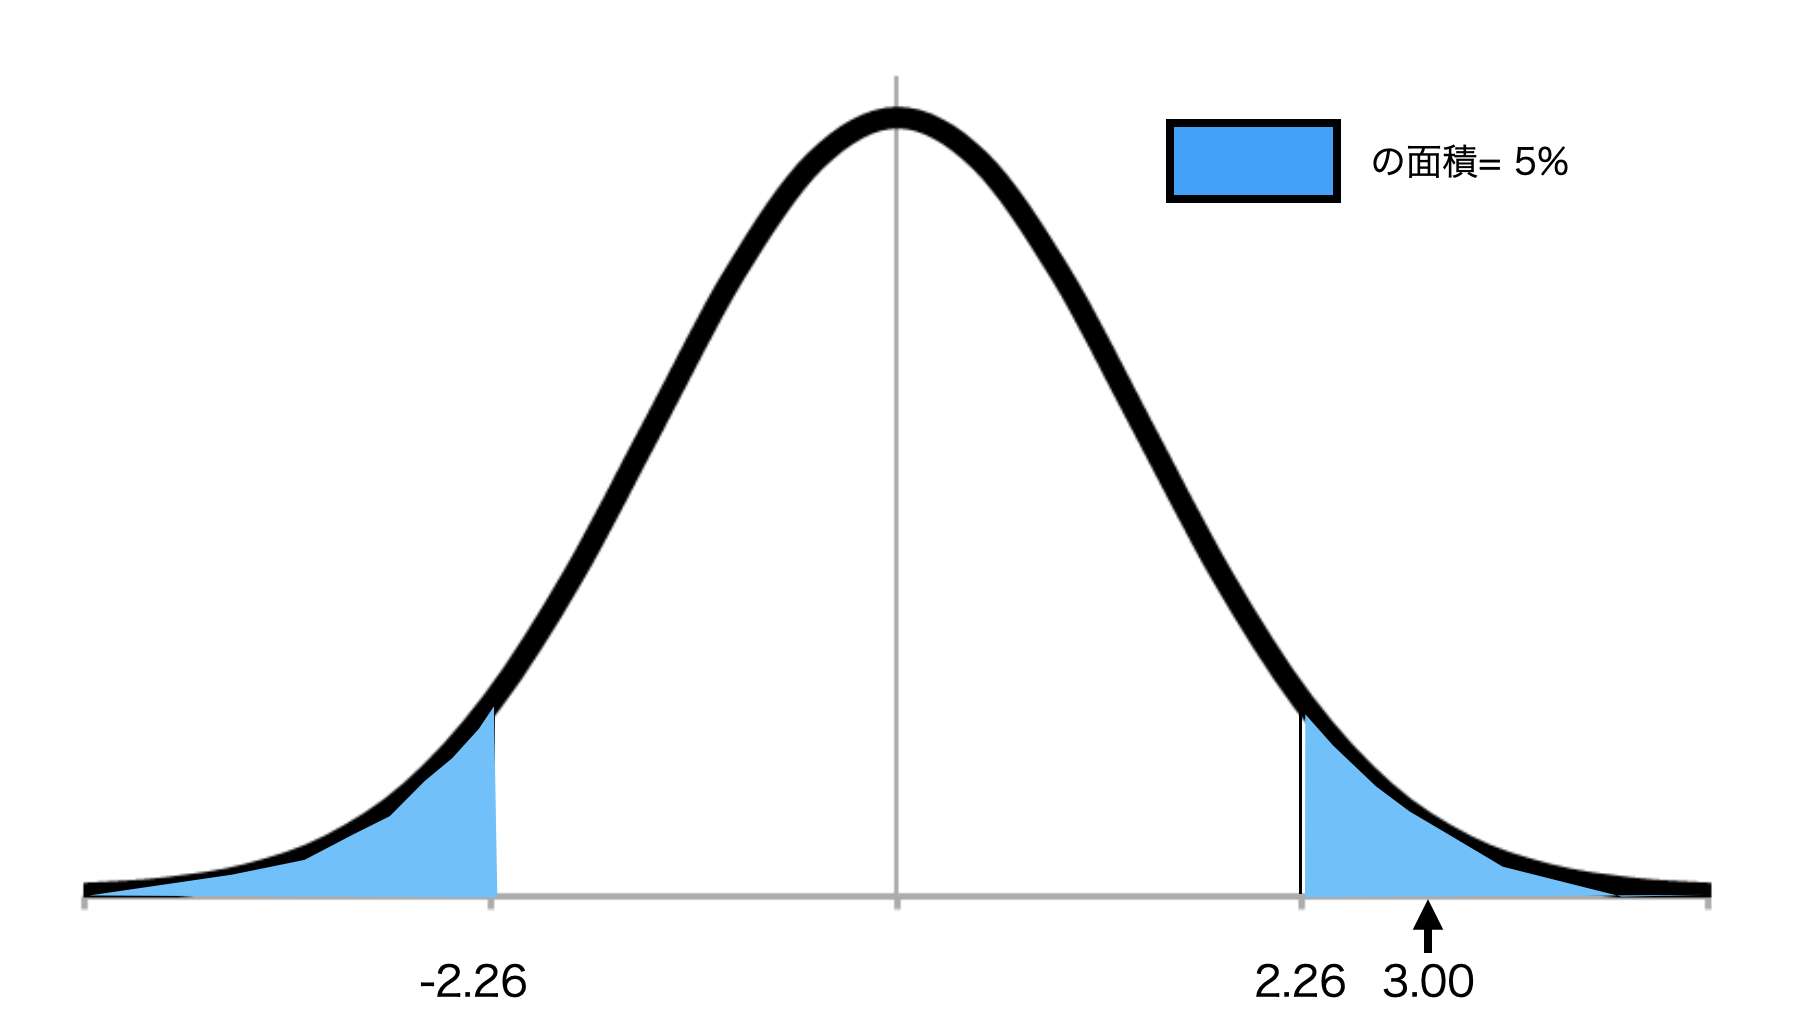
\includegraphics[width=10cm]{../pics/kasetsu.png}
  \caption{t分布による仮説検定}
  \label{fig:kasetsu}
\end{figure}

\newpage

次に, 回帰の有意性, 言い換えると, 取り上げた説明変数$x_1, \cdots, x_p$が全体として$y$の予測に役立つと言えるのかどうかの検定問題を考える. まず, 予測値$Y_i$は指定変数の組$(x_{1i}, x_{2i}, \cdots, x_{pi})$に対して
\begin{align}
  \label{eq:prediction}
  Y_i = \hat{a}_0 + \hat{a}_1x_{1i} + \cdots + \hat{a}_px_{pi}
\end{align}
のように計算される. そして, 観測値$y_i$の変動(平方和)を式\eqref{eq:sum_of_square}のように分解する.
\begin{align}
  \notag
  \sum_{i=1}^n(y_i-\bar{y})^2 
  &= \sum_{i=1}^n(y_i-\bar{Y})^2 \\
  \notag
  &\text{\quad ($\because$ 
  \; $\bar{y}= \frac{1}{n}\sum_{i=1}^ny_i = \frac{1}{n}\sum_{i=1}^nY_i + \frac{1}{n}\sum_{i=1}^ne_i = \frac{1}{n}\sum_{i=1}^nY_i = \bar{Y}$より)} \\
  \notag
  &= \sum_{i=1}^n(y_i-Y_i + Y_i-\bar{Y})^2 \\
  \label{eq:sum_of_square}
  &= \sum_{i=1}^n(y_i-Y_i)^2+\sum_{i=1}^n(Y_i-\bar{Y})^2 +2\sum_{i=1}^n(y_i-Y_i)(Y_i-\bar{Y})
\end{align}
また, $\S1.5$で次のような関係となることがわかっている. 
\begin{align}
  \label{eq:ch5_19}
    \begin{cases}
      \displaystyle
      \sum_{i=1}^n  \left\{
      (y_i-\bar{y})-\hat{a}_1(x_{1i}-\bar{x}_1)-\hat{a}_2(x_{2i}-\bar{x}_2)-\cdots -\hat{a}_p(x_{pi}-\bar{x}_p)
    \right\} = 0 \\
    \displaystyle
    \sum_{i=1}^n  \left\{
      (y_i-\bar{y})-\hat{a}_1(x_{1i}-\bar{x}_1)-\hat{a}_2(x_{2i}-\bar{x}_2)-\cdots -\hat{a}_p(x_{pi}-\bar{x}_p)\right
    \}x_{1i} = 0 \\
    \qquad \vdots \\
    \displaystyle
    \sum_{i=1}^n  \left\{
      (y_i-\bar{y})-\hat{a}_1(x_{1i}-\bar{x}_1)-\hat{a}_2(x_{2i}-\bar{x}_2)-\cdots -\hat{a}_p(x_{pi}-\bar{x}_p)\right
    \}x_{ji} = 0\\
    \qquad \vdots \\
    \displaystyle
    \sum_{i=1}^n  \left\{
      (y_i-\bar{y})-\hat{a}_1(x_{1i}-\bar{x}_1)-\hat{a}_2(x_{2i}-\bar{x}_2)-\cdots -\hat{a}_p(x_{pi}-\bar{x}_p)\right
    \}x_{pi} = 0
    \end{cases}
\end{align}

式\eqref{eq:ch5_19}を用いると, 式\eqref{eq:sum_of_square}の第3項は
\begin{align}
  \notag
    \sum_{i=1}^n(y_i-Y_i)(Y_i-\bar{Y}) 
    &= \sum_{i=1}^n\left\{
      y_i-(\hat{a}_0+\hat{a}_1x_{1i}+\cdots +\hat{a}_px_{pi})
    \right\}
    \left\{
      \hat{a}_0 +\hat{a}_1x_{1i}+\cdots \hat{a}_px_{pi}-\bar{Y}
    \right\} \\
    \notag
    &=\sum_{i=1}^n\left\{
      (y_i-\bar{y})-\hat{a}_1(x_{1i}-\bar{x}_1)-\cdots -\hat{a}_p(x_{pi}-\bar{x}_p)
    \right\}
    \left\{
      \hat{a}_0+\hat{a}_1x_{1i}+\cdots \hat{a}_px_{pi}-\bar{Y}
    \right\} \\
    \notag
    & \text{\quad ($\because$ 式\eqref{eq:sec5_y_bar}
    \; $\hat{a}_0 = \bar{y}-(\hat{a}_1\bar{x}_1+\cdots+\hat{a}_p\bar{x}_p)$より)} \\
    &= 0 
\end{align}
したがって, 式\eqref{eq:sum_of_square3}のように変動の分解ができる. 
\begin{align}
  \label{eq:sum_of_square3}
  \underbrace{\sum_{i=1}^n(y_i-\bar{y})^2}_{全変動(S_T)} = &\underbrace{\sum_{i=1}^n(Y_i-\bar{Y})^2}_{回帰変動(S_R)}+\underbrace{\sum_{i=1}^n(y_i-Y_i)^2}_{残差変動(S_e)}
\end{align}

右辺の第1項$\operatorname{S}_R$は回帰式に基づく予測値$Y_i$の変動, 第2項$\operatorname{S}_e$は残差の変動であって, 前者は全変動のうち回帰によって説明される部分, 後者は説明されない部分の変動である. もし取り上げた説明変数$x_1, \cdots, x_p$が$y$の予測に有効であるとすれば, 全変動$S_T$は一定であるため残差変動$S_e$は小さくなり, 逆に無効であるとすれば, $S_e$は大きくなる. ここで
\begin{align}
  \label{eq:coefficient_of_determination}
  \operatorname{R}^2 = \frac{\operatorname{S}_R}{\operatorname{S}_T} = \frac{\sum_{i=1}^n(Y_i-\bar{Y})^2}{\sum_{i=1}^n(y_i-\bar{y})^2}
\end{align}
のようにおけば, $\operatorname{R}^2$は全体の変動のうち回帰によって説明される部分の大きさの割合を表し, その意味で{\bf 決定係数}あるいは{\bf 寄与率}と呼ばれる. また, $\operatorname{S}_e$は最小化された予測誤差の平方和$\operatorname{F}(\hat{a}_0, \hat{a}_1, \cdots , \hat{a}_p)$に等しい.

そして, $\S1.7$で重相関係数$r_{y・12\cdots p}$は
\begin{align*}
  r_{y・12\cdots p} = \frac{s_{yY}}{\sqrt{s_{yy}s_{YY}}}
\end{align*}
のように表せた. これを2乗した式\eqref{eq:mul_correlation_coefi}を考える. 
\begin{align}
  \label{eq:mul_correlation_coefi}
  r_{y・12\cdots p}^2 
  &= \frac{s_{yY}^2}{s_{yy}s_{YY}} 
\end{align}
ここで, 
\begin{align}
  \notag
  s_{yY} &= \frac{1}{n}\sum_{i=1}^n(y_i-\bar{y})(Y_i-\bar{Y}) \\
  \notag
  &= \frac{1}{n}\sum_{i=1}^n(y_i-Y_i+Y_i-\bar{Y})(Y_i-\bar{Y}) \\
  \notag
  &= \frac{1}{n}\sum_{i=1}^n(e_i+Y_i-\bar{Y})(Y_i-\bar{Y}) \\
  \label{eq:cov_yY}
  &= \frac{1}{n}\sum_{i=1}^ne_i(Y_i-\bar{Y})+\frac{1}{n}\sum_{i=1}^n(Y_i-\bar{Y})^2 
\end{align}

\begin{itembox}[l]{残差の性質}
  残差$e_i = y_i - (a_0 + a_1x_{1i} + \cdots + a_px_{pi})$には次の2つの性質がある. 
  \begin{itemize}
    \item 残差の総和は0
    \begin{align}
      \label{eq:sum_ei}
      \sum_{i=1}^ne_i = 0
    \end{align}
    \item 説明変数$x_i$と残差$e_i$との積和は0
    \begin{align}
      \label{eq:sum_eixi}
      \sum_{i=1}^nx_{ji}e_i = 0
    \end{align}
  \end{itemize}
\end{itembox}

式\eqref{eq:cov_yY}の右辺第1項に関して, 
\begin{align}
  \notag
  \sum_{i=1}^ne_i(Y_i-\bar{Y})
  &= \sum_{i=1}^ne_iY_i-\bar{Y}\sum_{i=1}^ne_i  \\
  \notag
  &= \sum_{i=1}^ne_i(\hat{a}_0+\hat{a}_1x_{1i}+\cdots + \hat{a}_px_{pi}) \text{\quad ($\because$ 式\eqref{eq:sum_ei} \;$\sum_{i=1}^ne_i = 0$より)}\\
  \notag
  &= \hat{a}_0\sum_{i=1}^ne_i+\hat{a}_1\sum_{i=1}^ne_ix_{1i}+\cdots +\hat{a}_p\sum_{i=1}^ne_ix_{pi} \\
  \label{eq:residual_err}
  &= 0 
  \text{\quad ($\because$ 式\eqref{eq:sum_eixi} \;$\sum_{i=1}^nx_{ji}e_i = 0$より)}
\end{align}
したがって, 式\eqref{eq:cov_yY}は式\eqref{eq:residual_err}の結果から, 
\begin{align}
  \tag{\ref{eq:cov_yY}}
  s_{yY} 
  &= \frac{1}{n}\sum_{i=1}^ne_i(Y_i-\bar{Y})+\frac{1}{n}\sum_{i=1}^n(Y_i-\bar{Y})^2 \\
  \label{eq:syY2sYY}
  &= \frac{1}{n}\sum_{i=1}^n(Y_i-\bar{Y})^2 = s_{YY}
\end{align}
式\eqref{eq:syY2sYY}の結果より, $s_{yY}=s_{YY}$であるから, 式\eqref{eq:mul_correlation_coefi}は
\begin{align}
  \tag{\ref{eq:mul_correlation_coefi}}
  r_{y・12\cdots p}^2 
  &= \frac{s_{yY}^2}{s_{yy}s_{YY}} \\
  \notag 
  &= \frac{s_{YY}^2}{s_{yy}s_{YY}} \\
  \notag 
  &= \frac{s_{YY}}{s_{yy}} \\
  \notag 
  &= \frac{\sum_{i=1}^n(Y_i-\bar{Y})^2}{\sum_{i=1}^n(y_i-\bar{y})^2} \\
  \label{eq:r2_R2}
  &= \operatorname{R^2}
\end{align}
となり, 重相関係数$r_{y・12\cdots p}$の2乗は決定係数$\operatorname{R}^2$と等しくなる.  \\

\begin{itembox}[l]{$\chi^2$分布}
  $Z_1, Z_2, \cdots, Z_k$が互いに独立で標準正規分布$N(0, 1)$に従う確率変数であるとき, 次の式は{\bf $\chi^2$分布}に従うという. 
  \begin{align*}
    \chi^2 = Z_1^2 + Z_2^2 + \cdots + Z_k^2
  \end{align*}
\end{itembox}

モデルが適合しているとき$\sum(y_i-Y_i)^2/\sigma^2$は, 
\begin{align*}
  \sum(y_i-Y_i)^2/\sigma^2 = \sum(e_i-0)^2/\sigma^2
\end{align*}
となるので自由度$n-p-1$のカイ2乗分布に従う. また特に説明変数$x_1, \cdots, x_p$が$y$の予測に何ら寄与しない, 言い換えれば母集団における回帰係数の値が$a_1=\cdots = a_p=0$のときには, 
回帰の変動は
\begin{align*}
  \sum_{i=1}^{n}(Y_i-\bar{Y})^2
  &= \sum_{i=1}^{n}\left\{
    (\hat{a}_0 + \hat{a}_{1}x_{1i} + \cdots + \hat{a}_{p}x_{pi})
    - (\hat{a}_0 + \hat{a}_{1}\bar{x}_1 + \cdots + \hat{a}_{p}\bar{x}_p)
  \right\}^2 \\
  &= \sum_{i=1}^{n} \left\{
    \hat{a}_1(x_{1i}-\bar{x}_1) + \cdots + \hat{a}_p(x_{pi}-\bar{x}_p)
  \right\}^2 \\
  &= \sum_{i=1}^{n} \sum_{j=1}^p \hat{a}_j^2(x_{ji} - \bar{x}_{j})^2
  + \sum_{i=1}^n\sum_{j=1}^p\sum_{l=1}^p \hat{a}_j\hat{a}_l(x_{ji}-\bar{x}_{j})(x_{li}-\bar{x}_l) \qquad (j\neq l)\\
  &= n\sum_{j=1}^p \hat{a}_j^2s_{jj} 
  + n\sum_{j=1}^p\sum_{l=1}^p\hat{a}_j\hat{a}_ls_{jl} 
\end{align*}
$\operatorname{V}(\hat{a}_j)=\frac{\sigma^2}{ns_{jj}}$, かつ, 説明変数$x_j, x_l$は互いに独立であることを用いると, 
\begin{align*}
  \sum_{i=1}^{n}(Y_i-\bar{Y})^2
  &= \sum_{j=1}^p\frac{\hat{a}_j^2\sigma^2}{\operatorname{V}(\hat{a}_j)} \\
  \frac{1}{\sigma^2}\sum_{i=1}^{n}(Y_i-\bar{Y})^2 
  &= \sum_{j=1}^p\frac{\hat{a}_j^2}{\operatorname{V}(\hat{a}_j)} \\
  &= \sum_{j=1}^p\left( \frac{\hat{a}_j}{\sqrt{\operatorname{V}(\hat{a}_j)}} \right)^2
\end{align*}
$u = \frac{\hat{a}_j -a_j}{\sqrt{\operatorname{V}(\hat{a}_j)}}\sim \operatorname{N}(0, 1)$において, $a_j=0, j=1, \cdots, p$と仮定すると, 
\begin{align*}
  u= \frac{\hat{a}_j}{\sqrt{\operatorname{V}(\hat{a}_j)}} \sim \operatorname{N}(0, 1)
\end{align*}
なので, 
\begin{align*}
  \sum_{j=1}^p\left( \frac{\hat{a}_j}{\sqrt{\operatorname{V}(\hat{a}_j)}} \right)^2
\end{align*}
は自由度$p$の$\chi^2$分布に従う. すなわち,
\begin{align*}
  \sum_{i=1}^n\frac{(Y_i - \bar{Y})^2}{\sigma^2}
\end{align*}
は$\sum(y_i-Y_i)^2/\sigma^2$とは独立に自由度$p$の$\chi^2$分布に従う.これより次のような分散分析表(表\ref{tab:anovo_table})が構成される. 

\begin{table}[htb]
  \centering
  \caption{分散分析表}
  \label{tab:anovo_table}
  \begin{tabular}{ccccc}\bhline{1.5pt}
   変動要因 &平方和 &自由度 &不偏分散 &分散比  \\ \hline
   回帰による &$\displaystyle \operatorname{S}_R=\sum_{i=1}^n(Y_i-\bar{Y})^2$ &$p$ &$\displaystyle \operatorname{V}_R = \frac{\operatorname{S}_R}{p}$ &$\displaystyle \operatorname{F}_0=\frac{\operatorname{V}_R}{\operatorname{V}_e}$  \\
   回帰からの &$\displaystyle \operatorname{S}_e=\sum_{i=1}^n(y_i-Y_i)^2$ &$n-p-1$ &$\displaystyle \operatorname{V}_e=\frac{\operatorname{S}_e}{n-p-1}$ & \\
   全体 &$\displaystyle \operatorname{S}_T=\sum_{i=1}^n(y_i-\bar{y})^2$ &$n-1$ & & \\ \hline
  \end{tabular}
\end{table}

この分散分析表において分散比$\operatorname{F}_0$が$\operatorname{F}_0\geq \operatorname{F}^p_{n-p-1}(\alpha)$ならば仮説$H_0: a_1=\cdots =a_p=0$は危険率$\alpha$で棄却され, 回帰が変動の大きな要因となっている(回帰が有意である)ため, 取り上げた説明変数は全体として$y$の予測に役立つ, と結論づけられる. ここで, $\operatorname{F}^p_{n-p-1}(\alpha)$は自由度$(p, n-p-1)$のF分布の上側$100\alpha\%$点である. 

\begin{itembox}[l]{F分布}
  \quad
  2つの確率分布$U, V$が次の条件を満たすとする. 
  \begin{description}
    \item[(i)] $U$は自由度$k_1$のカイ2乗分布$\chi^2(k_1)$に従う
    \item[(ii)] $V$は自由度$k_2$のカイ2乗分布$\chi^2(k_2)$に従う
    \item[(iii)] $U, V$は独立である. 
  \end{description}
  ここで, $U$と$V$をそれぞれの自由度で割って調整したあとにとった比, すなわちフィッシャー分散比を
  \begin{align*}
    \operatorname{F} = \frac{U/k_1}{V/k_2}
  \end{align*}
  と定義すると, $\operatorname{F}$が従う確率分布を自由度$(k_1, k_2)$のF分布といい, $\operatorname{F}_n^{k_1}$または$\operatorname{F}(k_1, k_2)$と表す. \\

  \quad 例えば, 回帰の自由度が3で残差の自由度が11であり, 分散比$\operatorname{F}_0=8.21$の場合, $\operatorname{F}_0 \geq \operatorname{F}_{11}^3(0.01)=6.217$となり, 仮説$\operatorname{H}_0: a_1=a_2=a_3=0$は危険率$1\%$で棄却され, 取り上げた3つの説明変数は$y$の予測に役立つと言える. (図\ref{fig:f})
\end{itembox}

\begin{figure}[phtb]
  \centering
  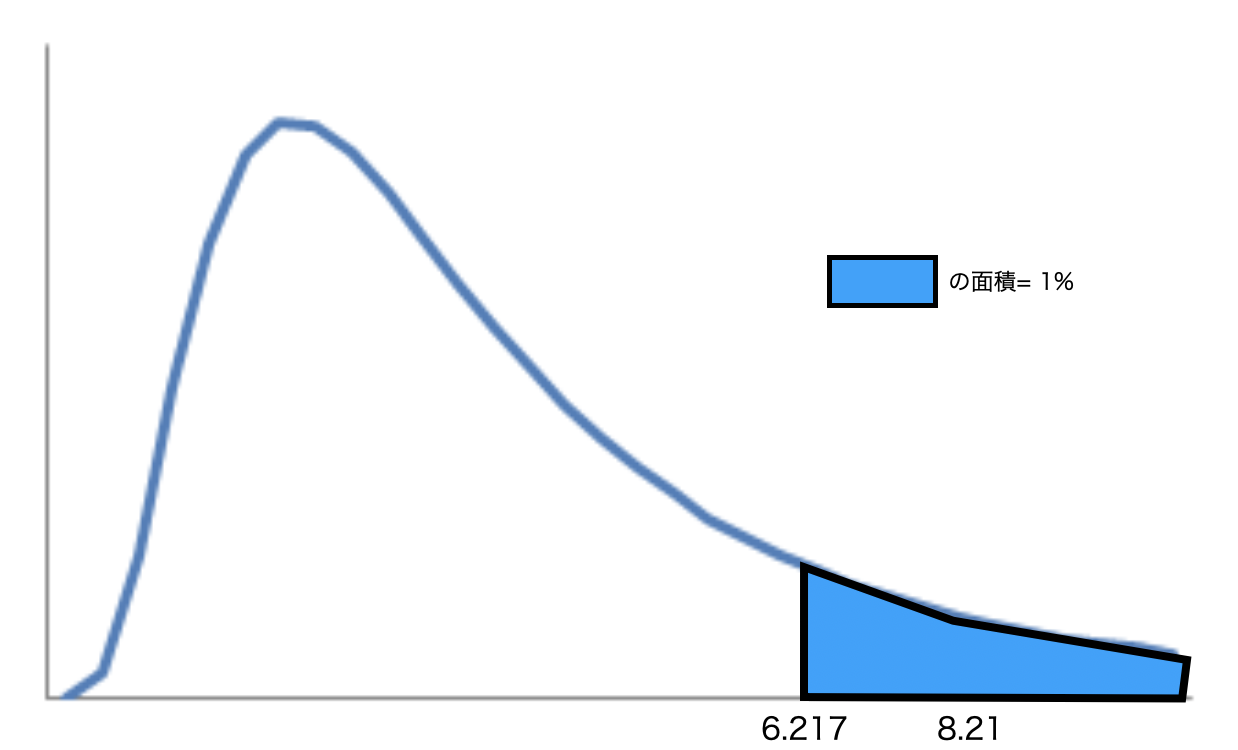
\includegraphics[width=10cm]{../pics/f.png}
  \caption{F検定}
  \label{fig:f}
\end{figure}

\newpage